

\chapter{التصميم البرمجي والتنجيز}
نبيّن في هذا الفصل التصميم البرمجي للنظام وطريقة تنجيزه والأدوات المستخدمة لذلك.
ونقوم بشرح مخططات الصفوف للحزم البرمجية.
وسرد القرارات التصميمة المعتبرة والأنماط التصميمية \eng{Design Patterns} المستخدمة.





\section{قراءة المعطيات}
تم بناء الحزمة \eng{datasets} للتعامل مع المعطيات. أي لقراءة النصوص وكتابة الميزات.
تحوي هذه الحزمة صف وحيد \eng{Document} وهو الصف الأساسي المستخدم ليحمل معلومات النص مثل اسمه ومساره وغيرها.
يبيّن الشكل~\ref{fig:cd:datasets} مخطط الصفوف لهذه الحزمة.
كما تحوي هذه الحزمة حزمتين جزئيتين هما الحزمة \eng{corpora} والحزمة \eng{writers}.

\begin{figure}[htb]
	\centering
	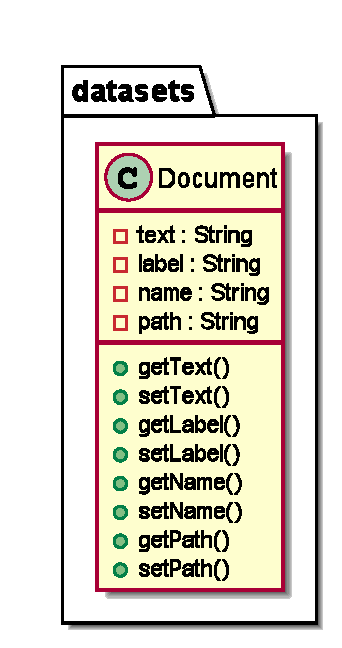
\includegraphics[width=0.25\linewidth]{images/cd-datasets.eps}
	\caption{%
		مخطط الصفوف للحزمة \eng{datasets}.
	}
	\label{fig:cd:datasets}
\end{figure}

الحزمة \eng{corpora} فيها مجموعة من الصفوف المستخدمة لقراءة مجموعة كبيرة من النصوص والمرور عليها ومعالجتها.
إذ أن الصفوف خارج هذه الحزمة تستخدم الواجهة \eng{TextCorpus}.
ويمكن توسيع هذه الحزمة بإنشاء صف جديد ينجّز هذه الواجهة.
حيث يجب أن يعرّف آلية الحصول على النصوص المكتوبة وتصنيفاتها.
تم استخدام النمط \eng{Iterator design pattern} لتحقيق ذلك.
إذ وجدناه مناسباً ويقوم بتأدية الغرض اللازم.
يبيّن الشكل~\ref{fig:cd:corpora} مخطط الصفوف لهذه الخزمة.

\begin{figure}[htb]
	\centering
	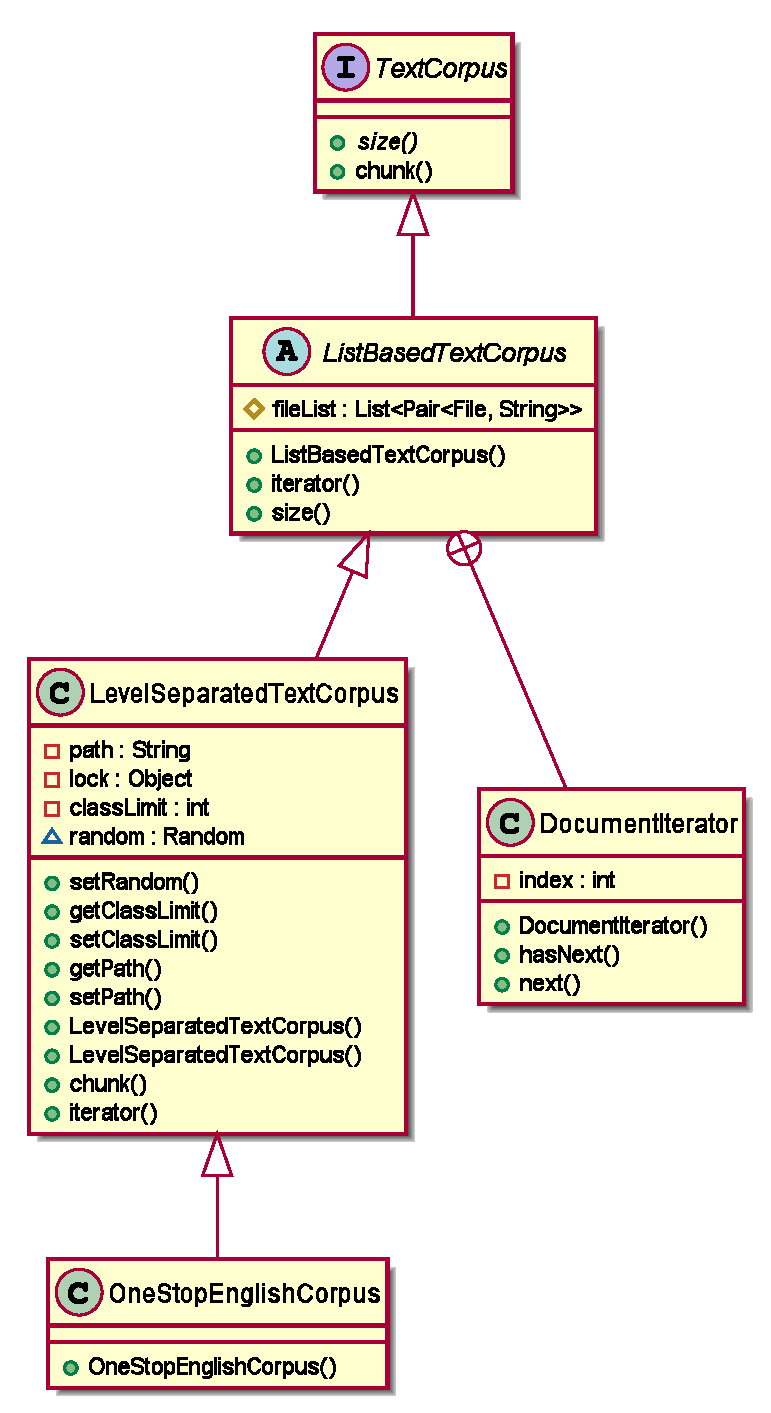
\includegraphics[width=0.6\linewidth]{images/cd-corpora.eps}
	\caption{%
		مخطط الصفوف للحزمة \eng{datasets.corpora}.
	}
	\label{fig:cd:corpora}
\end{figure}

وتم بناء الحزمة \eng{writers} لكتابة ملف فيه الميزات التي تم استخراجها من هذه النصوص.
يبيّن الشكل~\ref{fig:cd:writers} مخطط الصفوف لهذه الحزمة.
الواجهة الأساسية التي يتم استخدامها خارج هذه الحزمة هي \eng{FeatureWriter}.
الصف المكتوب والذي ينجزها يقوم بكتابة الميزات على ملف بلاحقة \eng{CSV (Comma Separated Values)}.
يمكن بإضافة صف ينجز هذه الواجهة تعريف آلية لكتابة الميزات بأي صيغة أخرى بحسب المطلوب كـ \eng{XML} مثلاً.

\begin{figure}[htb]
	\centering
	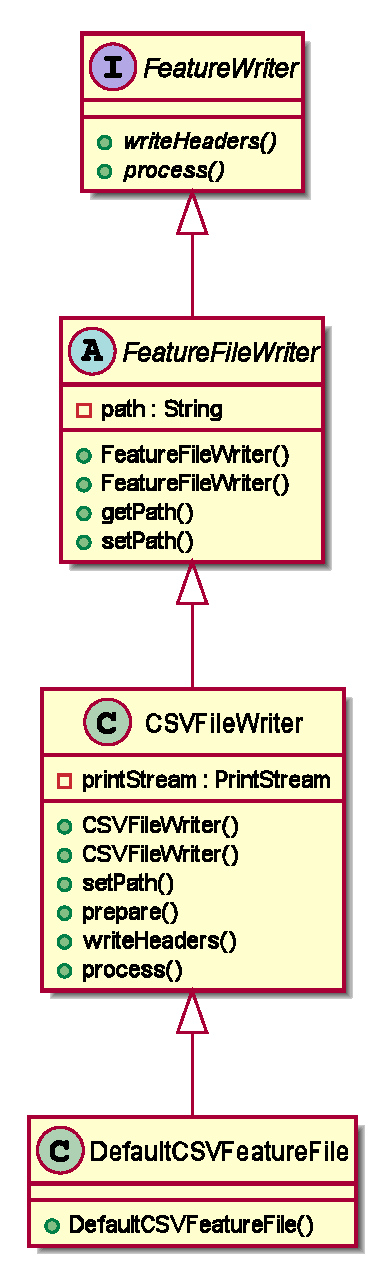
\includegraphics[width=0.25\linewidth]{images/cd-writers.eps}
	\caption{%
		مخطط الصفوف للحزمة \eng{datasets.writers}.
	}
	\label{fig:cd:writers}
\end{figure}

\afterpage{\clearpage}






\section{استخراج الميزات}
تم بناء الحزمة \eng{featureengineering} لتحوي الصفوف المسؤولة عن استخراج الميزات من النصوص.
تحوي هذه الحزمة صف واحد وأربع حزم جزئية.
الصف الموجود \eng{TextFeatureEngineer} هو صلة وصل،
إذ يقوم باستخدام الصف اللازم لقراءة النصوص واستخراج الميزات منها ثمّ كتابة ملف الميزات.
وأثناء عمله يقوم بطباعة معلومات مفيدة.
مثل اسم ورقم الملف الذي تتم معاجته حالياً، والوقت المُستغرَق للمعالجة.
وبعد الانتهاء يذكر عدد الملفات الذي حدث خطأ أثناء معالجتها.
ننوه إلى أن تنفيذ عملية استخراج الميزات تستهلك وقت يتراوح بين ساعة وساعتين.
والسبب الأساسي في استهلاك هذا الوقت الكبير هو استخدام مكتبات معالجة اللغات الطبيعية.
يوضح الشكل~\ref{fig:cd:featureengineering} مخطط الصفوف لهذه الحزمة.

\begin{figure}[htb]
	\centering
	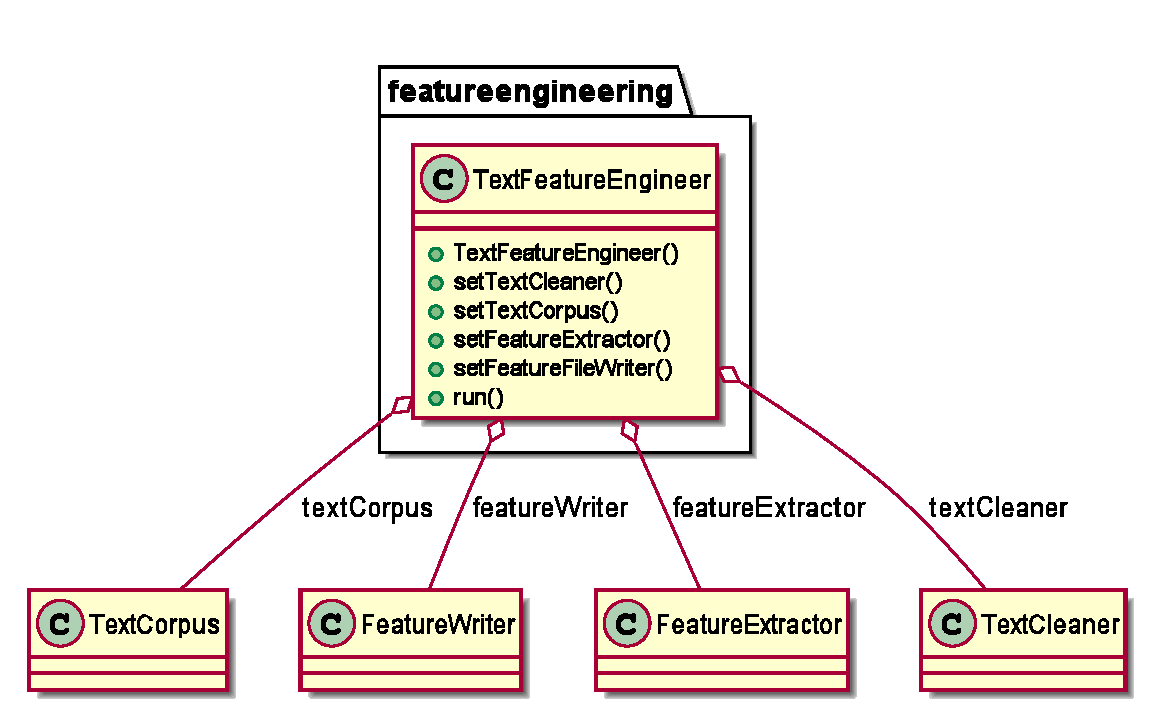
\includegraphics[width=0.8\linewidth]{images/cd-featureengineering.eps}
	\caption{%
		مخطط الصفوف للحزمة \eng{featureengineering}.
	}
	\label{fig:cd:featureengineering}
\end{figure}




\subsection{الحزمة \eng{cleaners}}
تحوي هذه الحزمة على الصفوف التي تقوم بتنظيف النص بشكل آلي قبل البدء بعملية استخراج الميزات.
مثل أن يتم تحويل جميع الأحرف إلى حروف صغيرة، أو حذف علامات الترقيم، إلخ.
تم استخدام النمط \eng{Decorator design pattern}.
وذلك للسماح باستخدام عدّة صفوف تقوم بالتنظيف ودون تحديد عددها وبشكل سهل الاستخدام.
يبيّن الشكل~\ref{fig:cd:cleaners} مخطط الصفوف لهذه الحزمة.

\begin{figure}[htb]
	\centering
	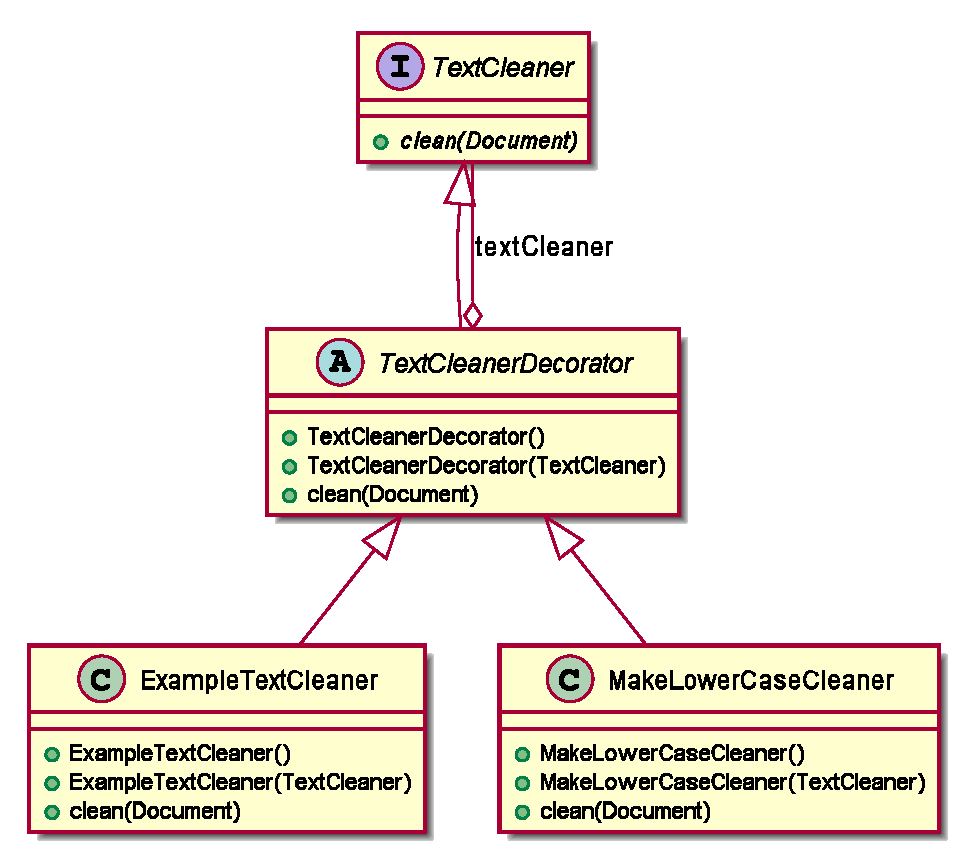
\includegraphics[width=0.75\linewidth]{images/cd-cleaners.eps}
	\caption{%
		مخطط الصفوف للحزمة \eng{featureengineering.cleaners}.
	}
	\label{fig:cd:cleaners}
\end{figure}




\subsection{الحزمة \eng{features}}
تحوي هذه الحزمة على الميزات التي تم تنجيزها.
كل صف يمثل ميزة.
وجميع هذه الصفوف تنجّز الواجهة \eng{Feature}.
ويمكن بإنشاء صفوف جديدة تُنجّز هذه الواجهة إضافة ميزات جديدة وتوسيع الحزمة.
يبيّن الشكل~\ref{fig:cd:features} جزء من مخطط الصفوف لهذه الحزمة.
نلاحظ أنه تم تقسيم الميزات بحسب طبيعتها إلى عدّة حزم جزئية.

\begin{figure}[htb]
	\centering
	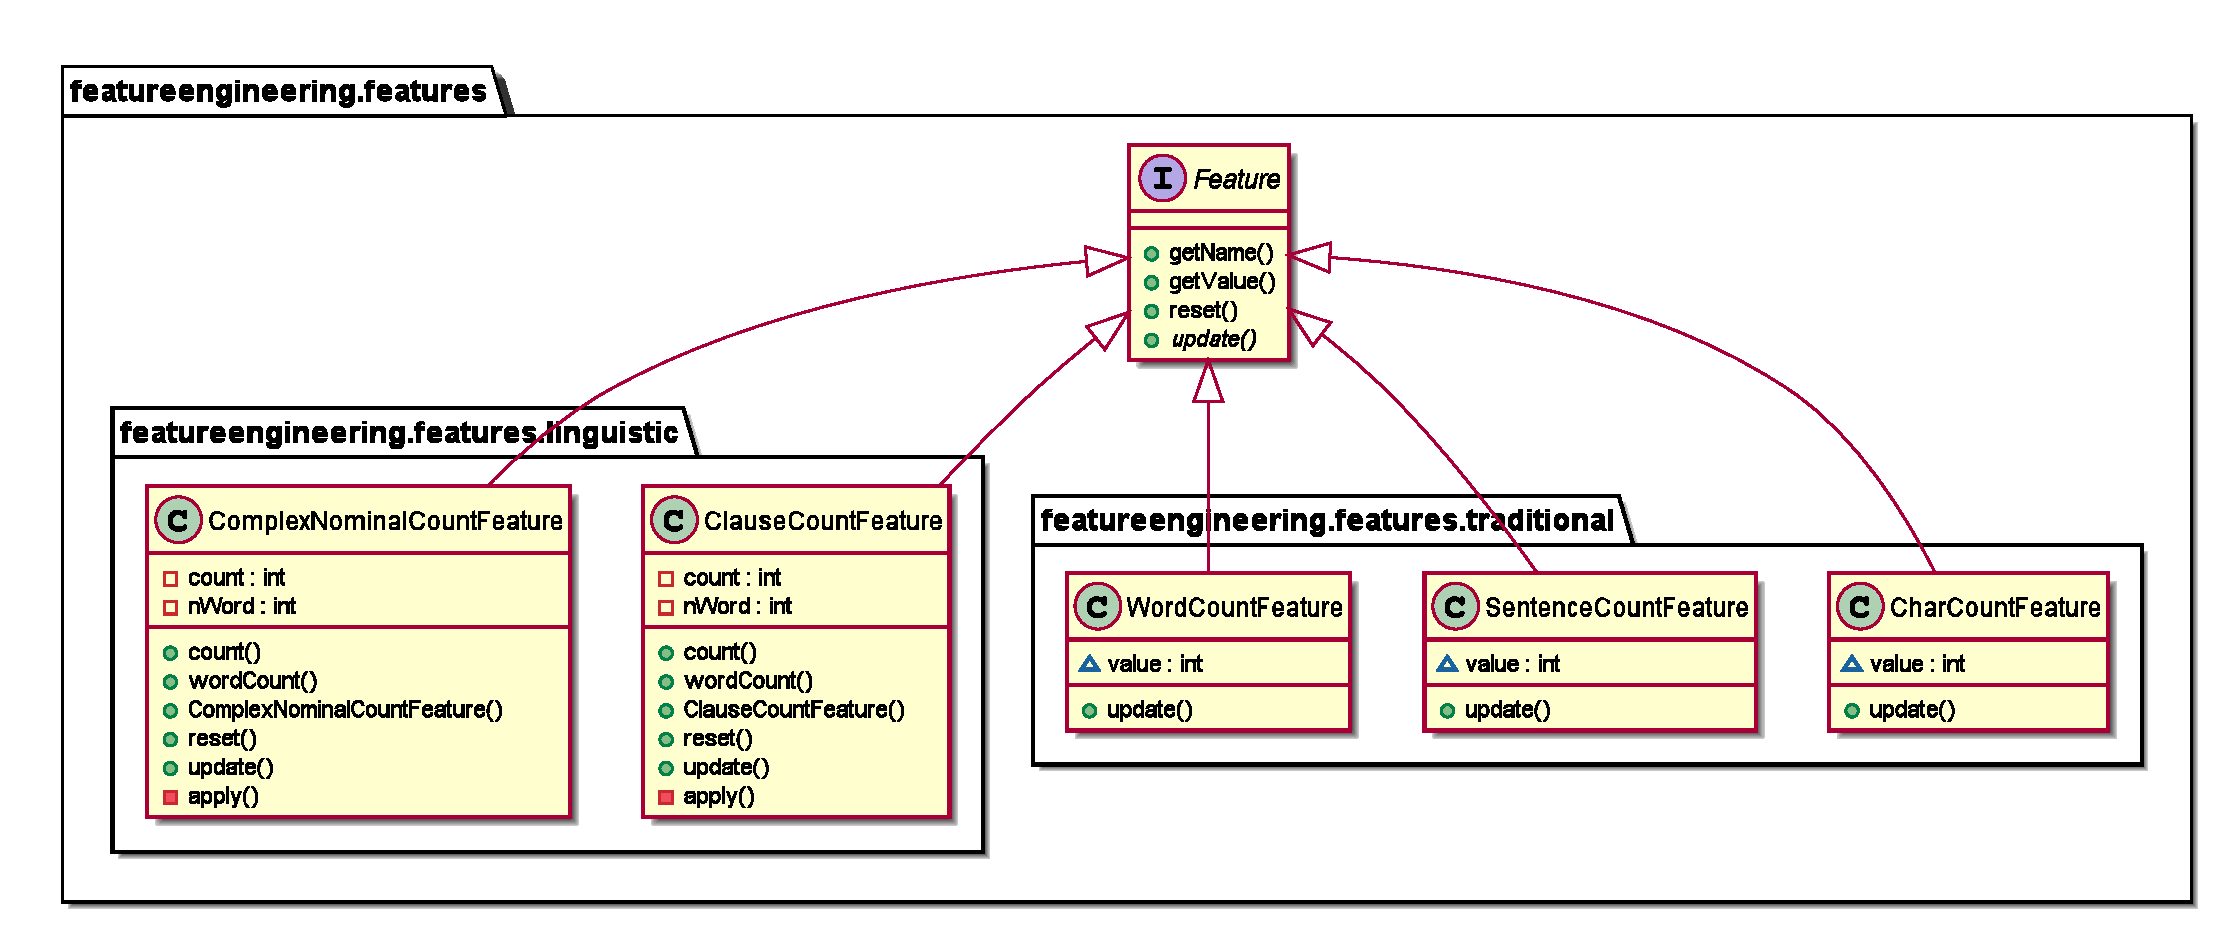
\includegraphics[width=0.95\linewidth]{images/cd-features.eps}
	\caption{%
		عيّنة من مخطط الصفوف للحزمة \eng{featureengineering.features}.
	}
	\label{fig:cd:features}
\end{figure}



\subsection{الحزمة \eng{featuresets}}
كل صف من صفوف هذه الحزمة يمثّل مجموعة ميزات مترابطة.
يبيّن الشكل~\ref{fig:cd:featuresets} عيّنة جزئية من مخطط الصفوف لهذه الحزمة.
الهدف من هذه الصفوف هو تسهيل استخدام الميزات التي تم تنجيزها ضمن سياق آخر.
يمكن للمستخدم (المستخدم في هذه الحالة هو مبرمج) بإنشاء صف يُنجّز الواجهة \eng{FeatureSet}
واستخدام الميزات التي يريدها من الحزمة \eng{features}.
أيضاً وجود هذه الصفوف يسمح بتركيب عدد من الميزات؛
فمثلاً يمكن استخدام الصف \eng{WordCountFeature} لحساب عدد الكلمات ضمن النص،
واستخدام الصف \eng{SentenceCountFeature} لحساب عدد الجمل،
ثمّ حساب متوسط طول الجملة بتقسيم عدد الكلمات على عدد الجمل.
تم استخدام هذا التصميم لفصل الميزات عن بعضها بحيث تكون مستقلة ويمكن استخدام كل منها على حدا،
وأيضاً لتفادي إعادة الحسابات ورفع الكفاءة.


\begin{figure}[htb]
	\centering
	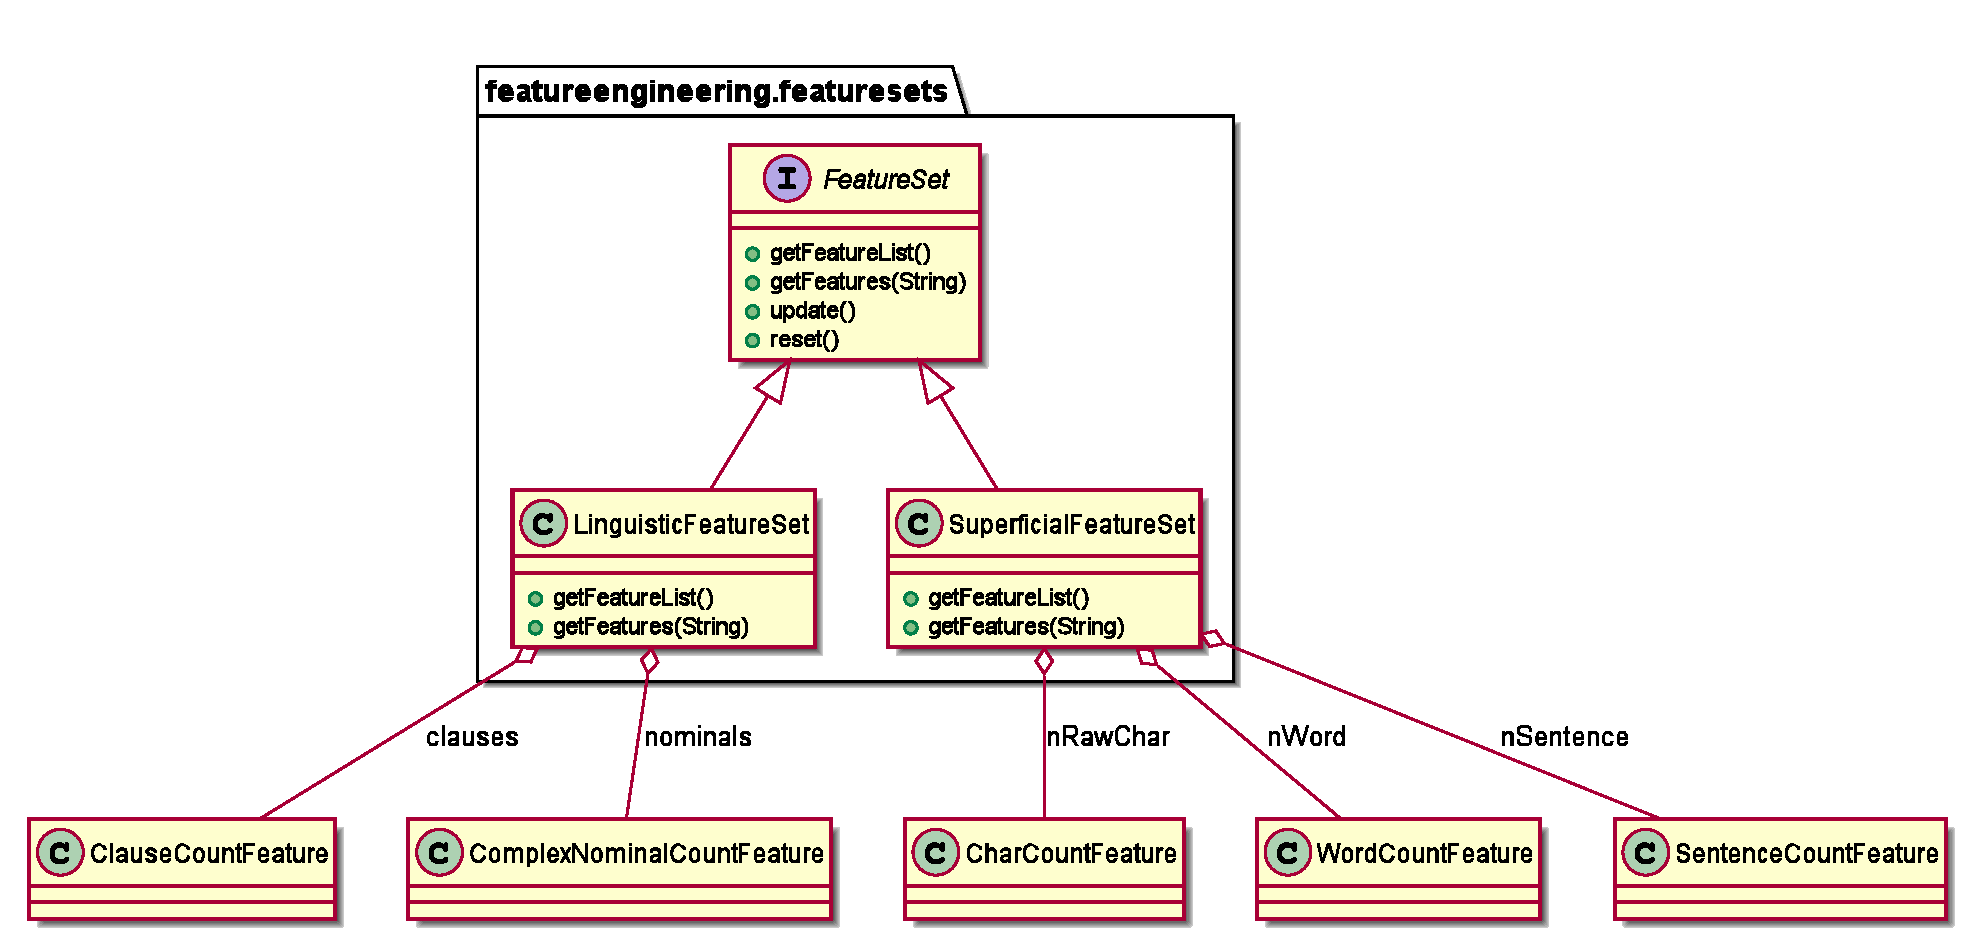
\includegraphics[width=0.95\linewidth]{images/cd-featuresets.eps}
	\caption{%
		عيّنة من مخطط الصفوف للحزمة \eng{featureengineering.featuresets}.
	}
	\label{fig:cd:featuresets}
\end{figure}



\subsection{الحزمة \eng{extractors}}
يبيّن الشكل~\ref{fig:cd:extractors} مخطط الصفوف لهذه الحزمة.
المكون الأساسي فيها هو الواجهة \eng{FeatureExtractor}.
إذ يعتبر المكوّن الأساسي في عملية استخراج الميزات.
له التابعين
\eng{getFeatureList()}
الذي يعيد أسماء الميزات.
والتابع
\eng{extract(String)}
الذي يعيد قيمة الميزات التي تم استخراجها للنص.
يمكن تنجيز هذه الواجهة بعدّة طرق.

الصف الذي تم إنشائه لتنجيز هذه الواجهة يستخدم النمط \eng{Observer design pattern}.
وهو الصف \eng{ObservableFeatureExtractor}.
يحوي هذا الصف على مجموعة من الـ \eng{FeatureSet} كل منها هو \eng{Observer}.
تم استخدام هذا النمط لكون عملية إعراب النص \eng{parsing}
باستخدام مكتبة معالجة اللغات الطبيعية يستهلك وقت (حوالي 6 ثواني للنص الواحد).
فبعد عملية الإعراب يقوم الصف بتنبيه مجموعات الميزات هذه والتي تقوم بدورها بتنبيه الميزات فتتحدث قيمها بحسب التغيير الجديد.

\begin{figure}[htb]
	\centering
	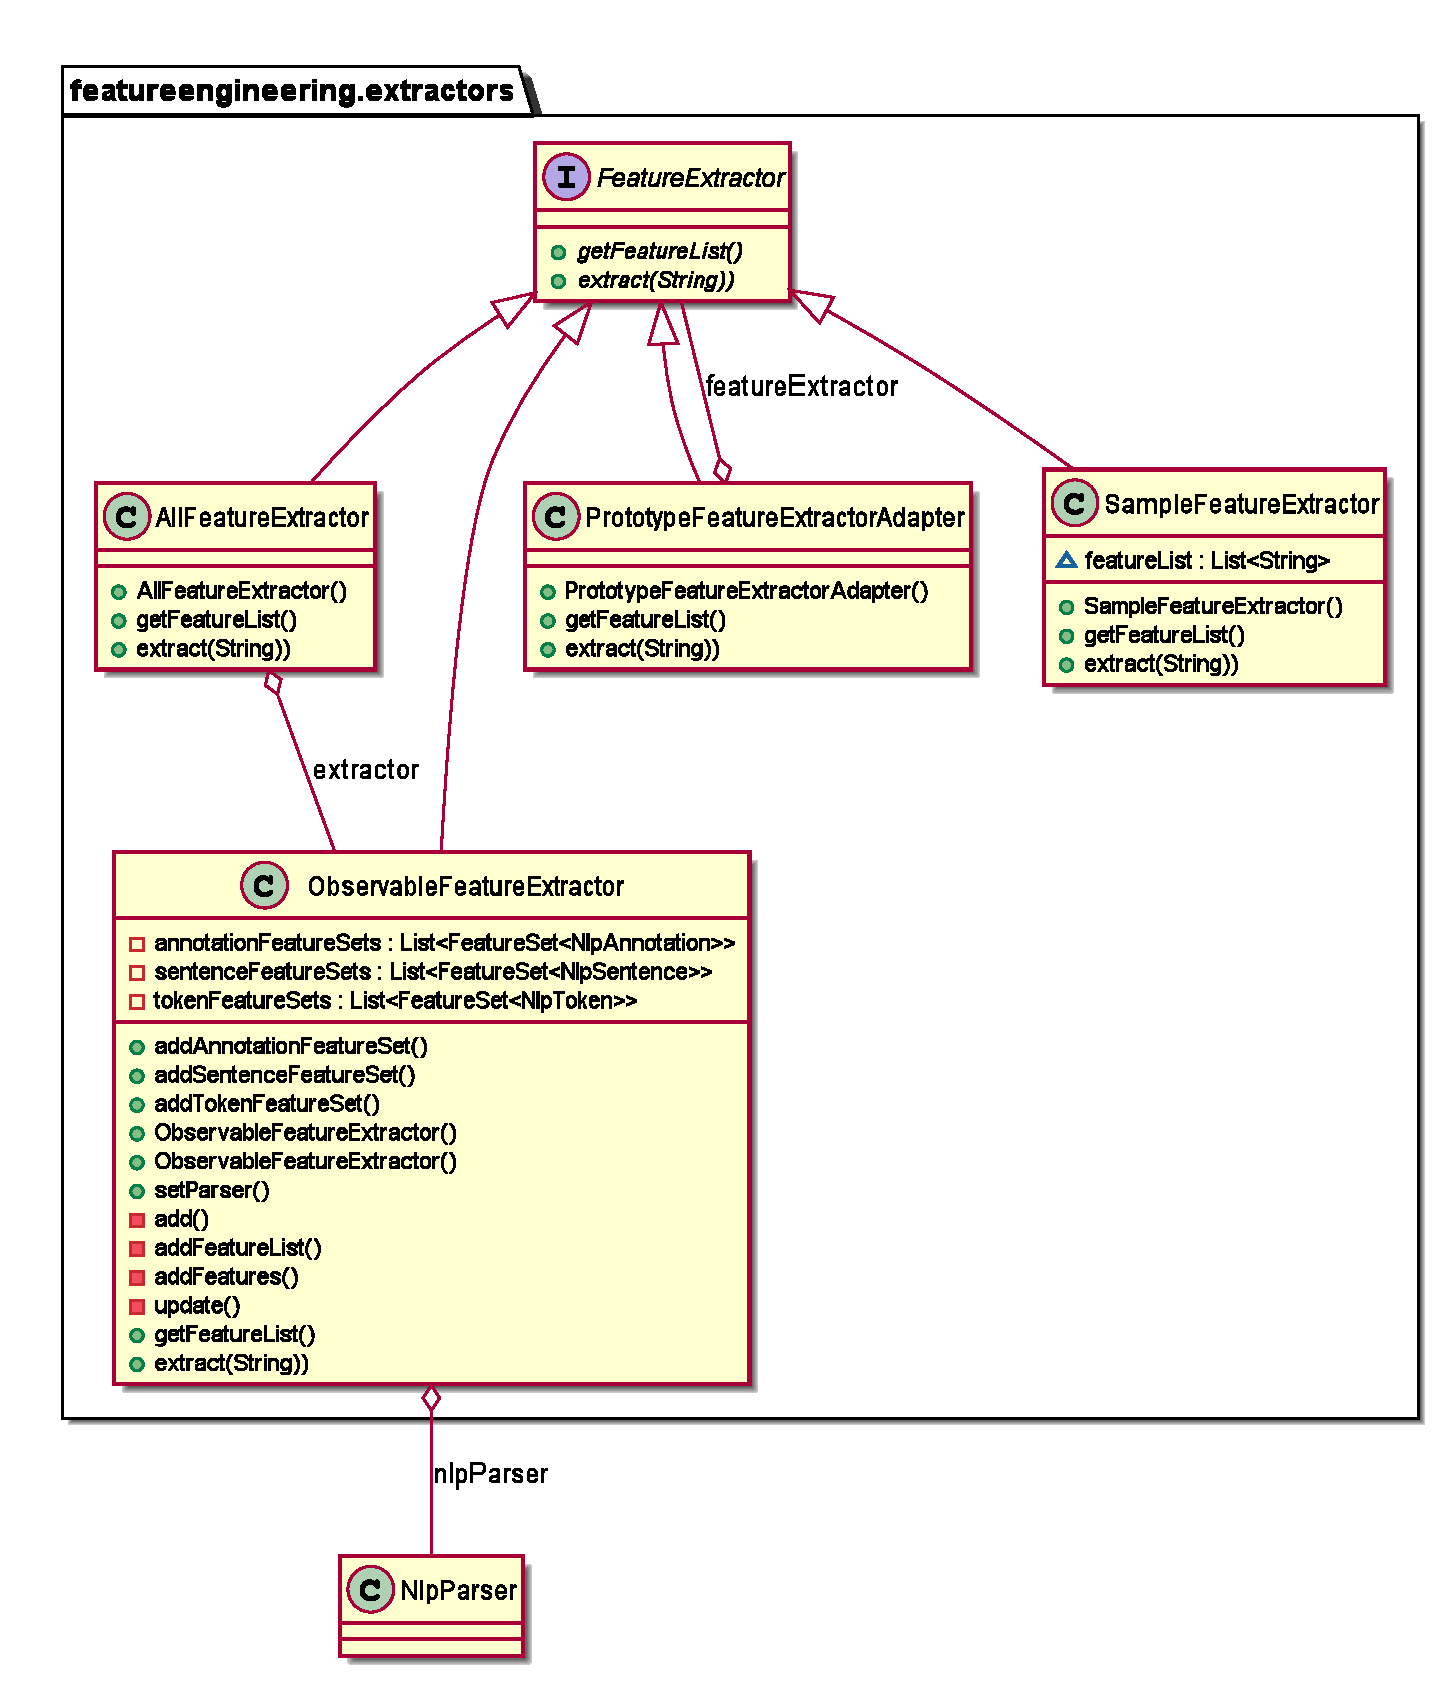
\includegraphics[width=0.8\linewidth]{images/cd-extractors.eps}
	\caption{%
		مخطط الصفوف للحزمة \eng{featureengineering.extractors}.
	}
	\label{fig:cd:extractors}
\end{figure}



\subsection{الحزمة \eng{nlp}}
تم بناء هذه الحزمة لتغليف وتوحيد الواجهة البرمجية \eng{API} لمكتبات معالجة اللغات الطبيعية.
فلقد استخدمنا في هذا المشروع مكتبة ستانفورد
\eng{Stanford Parser%
	\footnote{
		\url{https://nlp.stanford.edu/software/lex-parser.shtml}
	}
}
لذلك.
فهي مكتوبة بلغة جافا.
سهلة الاستخدام.
تقدم جميع الحسابات المطلوبة،
ولكنها تستغرق وقت كبير.
وإن تصميم الحزمة \eng{nlp} بهذا الشكل يسمح بتغيير المكتبة المستخدمة لمعالجة اللغات الطبيعية دون أي تغيير على باقي المكونات البرمجية.

تم استخدام النمط \eng{Adapter design pattern} لتحقيق ذلك.
إذ تم تعريف الواجهات الأساسية والتوابع الأساسية.
ولاستخدام مكتبة محددة نقوم بتنجيز الواجهات السابقة بحسب الواجهة البرمجة \eng{API} للمكتبة المستخدمة.
فبذلك تم عزل المكتبة المستخدمة عن الكود البرمجي المكتوب.
يوضح الشكل~\ref{fig:cd:nlp} عيّنة من مخطط الصفوف لهذه الحزمة.

\begin{figure}[htb]
	\centering
	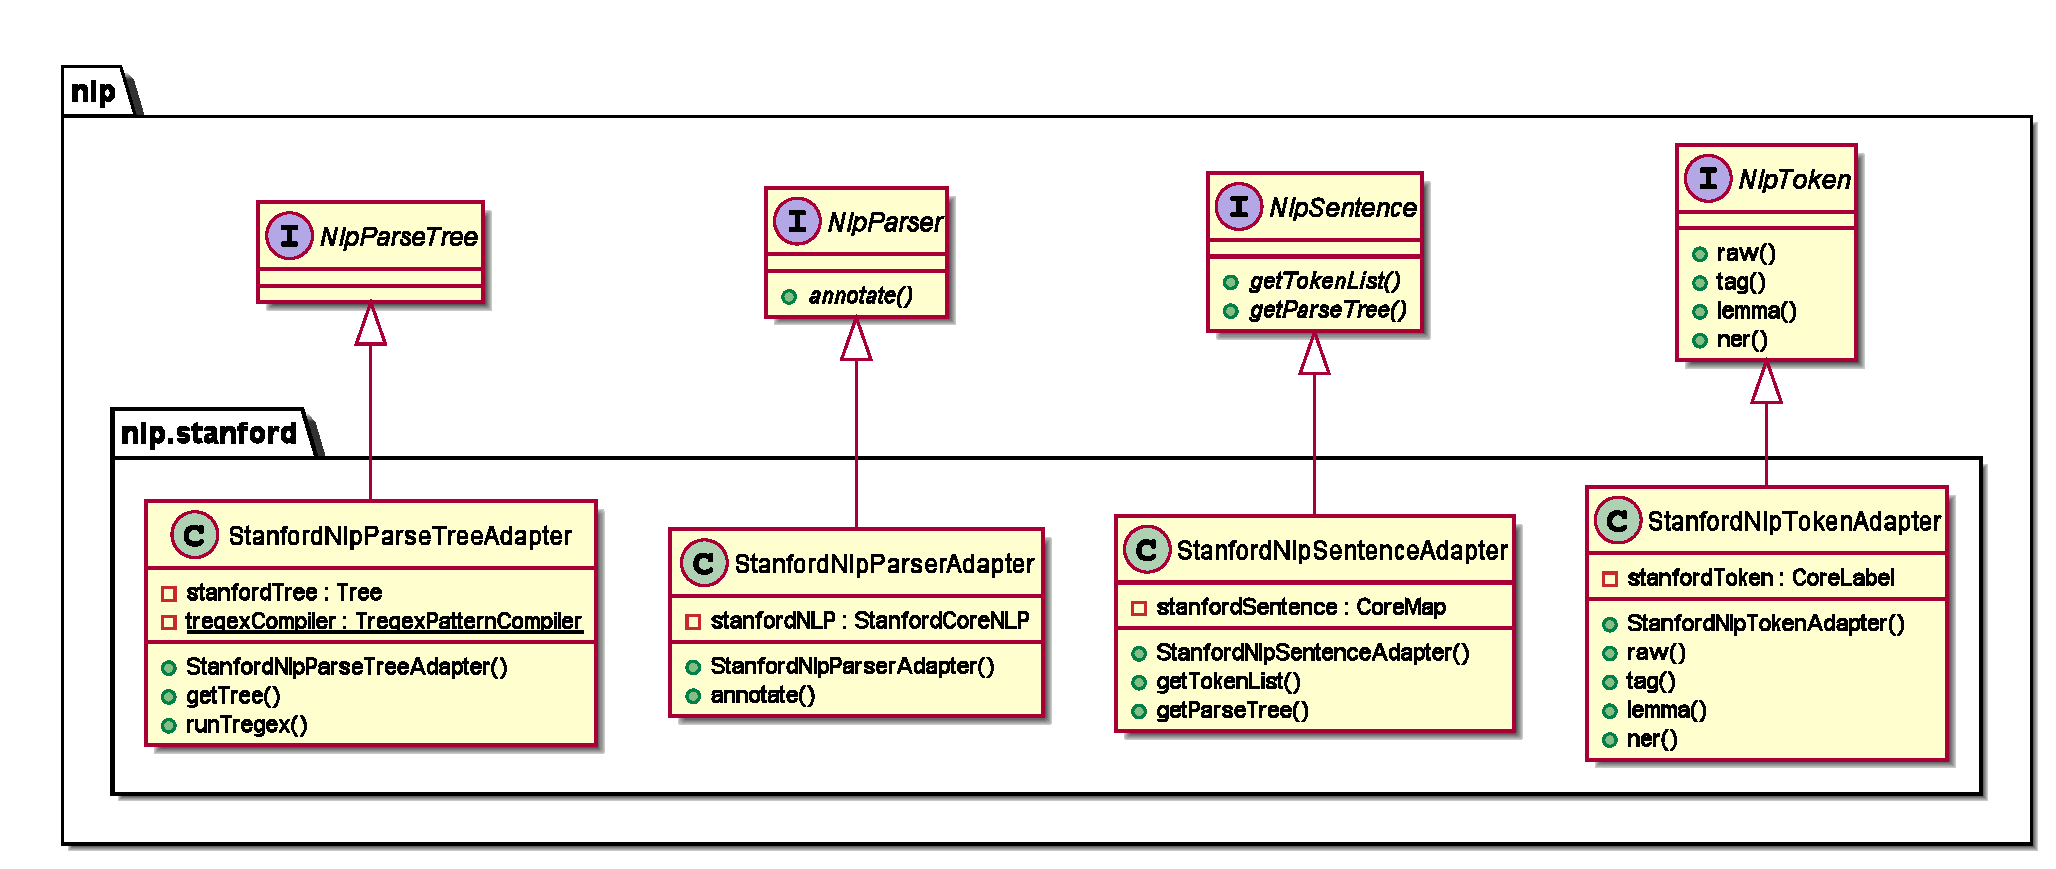
\includegraphics[width=1\linewidth]{images/cd-nlp.eps}
	\caption{%
		عيّنة من مخطط الصفوف للحزمة \eng{nlp}.
	}
	\label{fig:cd:nlp}
\end{figure}

\afterpage{\clearpage}



\section{خوارزميات تعلم الآلة}
توجد العديد من الأدوات \eng{tools} التي تقدم مجموعة واسعة من الوظائف لتطبيق خوارزميات ومفاهيم تعلم الآلة المختلفة.
ضمن هذا المشروع، تم اختيار الأداة \eng{Weka} لذلك.
todo





